\chapter{Classical Numerical Pricing Methods and Closed Form Solutions} % Main chapter title

\label{Chapter3} % Change X to a consecutive number; for referencing this chapter elsewhere, use \ref{ChapterX}

In last section we saw that the American put was an example of an option that requires numerical procedures to be priced fairly. The American put is far from the only example of a derivative without a closed form solution. We will look at two classical valuation algorithms for pricing American options in computational finance; the Cox-Ross-Rubinstein (CRR) binomial model and the least squares Monte Carlo method (LSM). The binomial model is an example of a strategy to approximate the option by discretization of the underlying risky asset(s) and the LSM is a method to simulate the underlying risky asset(s). Another popular choice is to solve the free-boundary problem with finite difference methods, but we choose to focus on the two other numerical procedures. The chapter will also investigate valuing exotic multivariate contingent claims. We extend the binomial pricing model \parencite{NEK,BEG} and LSM to multivariate contingent claims and provide some closed form solutions for exotic European options \parencite{Johnson87, Ouwehand2006}. Therefore the chapter has two purposes; to gain insight into valuation for exotic options and provide benchmarks for the neural networks in the coming chapters.

%----------------------------------------------------------------------------------------
%	SECTION 1
%----------------------------------------------------------------------------------------
\section{Cox Ross Rubinstein Model}\label{CRR}
The classical binomial pricing model or the CRR model presented in this section is inspired by \parencite{CRR,Hull,finKont}. The CRR model will be used for pricing an American put and an European call option with one underlying stock and to build the foundation for pricing bivariate contingent claims \parencite{BEG}. The model provides an intuitive and easily implementable model for valuing European and American options. The binomial model has its limitations, because it is not suited for valuing path dependent options or options with several underlying factors for computational reasons. The key difference of the binomial model and the simulation approach is that the binomial model is a discrete time model, where the underlying stochastic process has two possible movements per time-step. \\

Assume a frictionless market and the underlying stochastic process follow a multiplicative binomial process in discrete time. We work with the financial market $(\Omega, \mathcal{F}, \mathbb{F}, P, B, S_1)$, where the filtration is generated by $\mathbb{F}= \sigma(\mathcal{F}_{t_n})_{n=0,1,\ldots, N}$ and the sigma algebra is chosen to be $\mathcal{F}=\mathcal{F}_{t_{N}}$. It is well known from discrete time arbitrage theory, that the binomial market model with two assets, where $u>1+r>d>0$ is an arbitrage-free and complete model. The $u$,$d$ and $r$ describe the evolution of the discrete stochastic process for the stock and the risk-free interest rate on the bank account. 
\begin{align*}
B(t_n)=B_{0}(t_{n-1}) \cdot \exp(\Delta t \cdot r) \quad where \ B(0)=1 \ and \ n=1, \ldots, N\\
S_{1}(t_n)=S_{1}(0)\prod_{j=1}^{n} Y_{j} \quad where \ Y_1,Y_2, \ldots, Y_N \ are \ i.i.d., \ S_1(0)>0
\end{align*}
Note that the interest rate is continuously compounded for computational convenience and the equidistant time step is $\Delta t=T/N$ (section \ref{DiscreteValueFramework} for notation). We assume that: \[ Y_j = \begin{cases} 
      u & with \ probability \ p \\
      d & with \ probability \ (1-p)
   \end{cases}
\]

Below, an illustration of a discrete multiplicative binomial process with two time-steps, where the binomial tree recombines\footnote{Henceforth a binomial recombining tree is referred to as a binomial lattice}.\\

\begin{figure}[H]
\centering
% Define styles for bags and leafs
\tikzstyle{bag} = [text width=2em, text centered]
\tikzstyle{end} = []
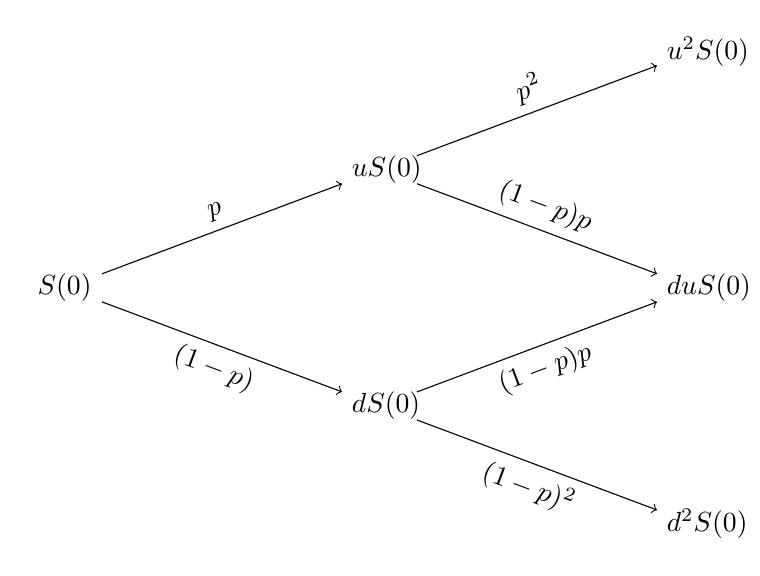
\begin{tikzpicture}[sloped]
   \node (a) at ( 0,0) [bag] {$S(0)$};
   \node (b) at ( 4,-1.5) [bag] {$d S(0)$};
   \node (c) at ( 4,1.5) [bag] {$u S(0)$};
   \node (d) at ( 8,-3) [bag] {$d^2 S(0)$};
   \node (e) at ( 8,0) [bag] {$d u S(0)$};
   \node (f) at ( 8,3) [bag] {$u^2 S(0)$};
   \draw [->] (a) to node [below] {$(1-p)$} (b);
   \draw [->] (a) to node [above] {$p$} (c);
   \draw [->] (c) to node [above] {$p^2$} (f);
   \draw [->] (c) to node [above] {$(1-p)p$} (e);
   \draw [->] (b) to node [below] {$(1-p)p$} (e);
   \draw [->] (b) to node [below] {$(1-p)^2$} (d);
\end{tikzpicture}
\decoRule
\caption[Two-dimensional Binomial Lattice]{Price dynamics of binomial lattice model with one underlying risky asset with N=2, $S(0)$ is spot value, p objective probability measure, u and d are realizations of the stochastic variable $Y_j$}
\label{fig:twoDimLattice}
\end{figure}

By constructing the discrete process for the stock it is easy to find the equivalent martingale measure. 
\begin{definition}\label{findQ}
Assume there exists a risk-free asset. A probability measure $Q$ is called a martingale measure if the following condition holds 
\begin{align*}
s= \exp(- r \Delta t) \cdot E^Q[S(t+\Delta t)|S(t)=s] 
\end{align*}
Where $\Delta t$ is a single time-step. \hfill (p. 18 \parencite{Bjork19})
\end{definition}
By using definition \ref{findQ} we find the risk neutral measure to be:
$$q=\frac{\exp(r \Delta t)-d}{u-d}$$
The martingale measure $q$ is unique in the binomial lattice model, because the model is complete. The pricing formula for a T-claim is given by the risk neutral valuation formula.
\begin{theorem}{\textbf{Risk neutral valuation formula (RVNF) in discrete time for a T-claim: }}\label{RNVF-Discrete}
The arbitrage-free price at t=0 of a T-claim $X$ is given by
\begin{align*}
\Pi(0;X)&= \exp(- r \Delta t \cdot N) \cdot E^Q[X]\\
&=\exp(- r \Delta t \cdot N) \cdot \sum_{n=0}^{N} \binom{N}{n} q^n (1-q)^{N-n} \Phi(su^n d^{N-n})
\end{align*}
Here, $Q$ denotes the martingale measure, $\Pi(0;X)$ is the price of X to time 0 and $\Delta t$ is a single time step. \\
\null \hfill (p. 25 \parencite{Bjork19})
\end{theorem}

Theorem \ref{RNVF-Discrete} gives a simple mathematical framework for pricing European options, but the model can readily be extended to American options. American put options for the binomial model will be solved with the dynamic programming approach. 
\begin{equation*}\label{BellmanEq2}
\begin{split}
\begin{cases}
          P(t_i) = max\{ (K-S(t_i))^+, \exp(-r\cdot \Delta t) E^Q[P(t_{i+1})|S(t_i)])\} \quad for \ i={0,\ldots,N-1} \\
          P(t_N) = (K-S(t_N))^+ 
\end{cases}
\end{split}
\end{equation*}
Note that the binomial lattice model has a recursive structure, where the one-step transition probabilities are the same in each node. At each exercise date, the idea is to either exercise to gain the intrinsic value if it is greater than the expected continuation value or hold the option alive for another period. The dynamic choice to exercise or to keep the option alive gives an exercise barrier $b$ (Figure \ref{fig:BinomialTree}).\\

\begin{figure}[th]
\centering
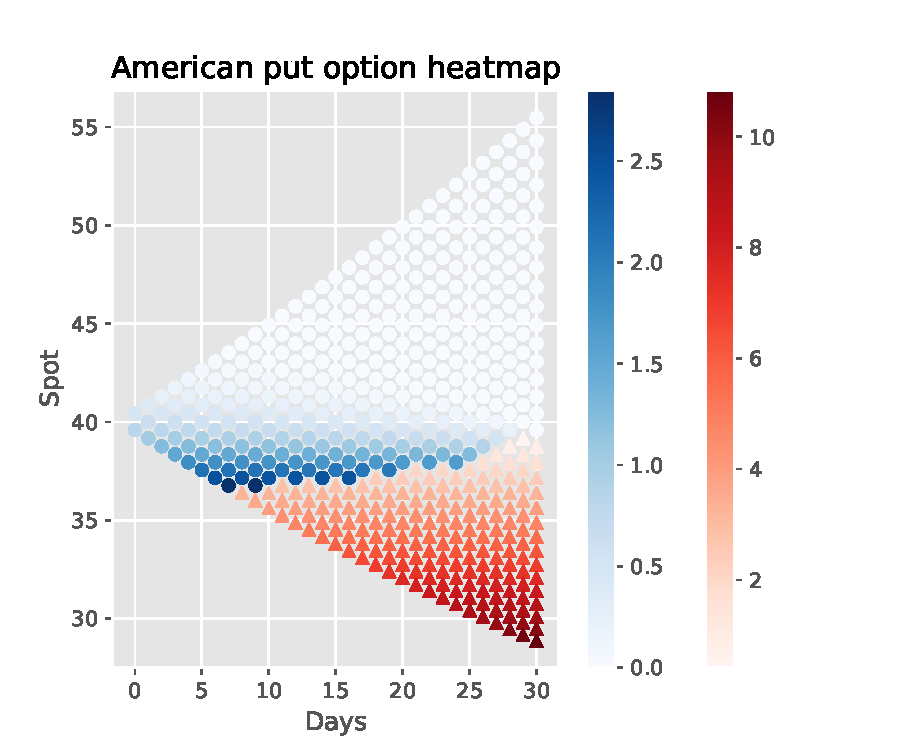
\includegraphics{Figures/BinomialTree.pdf}
\decoRule
\caption[Exercise Decisions Binomial Tree]{A valuation tree of an American put option price based on the binomial model, where the color indicates the value and the dots mark the continuation nodes. The parameters are S(0)=40, N=30, $\Delta t =$ 1 day, K=40 and u=1.0106}
\label{fig:BinomialTree}
\end{figure}

To value an American put option, we lay out all the possible paths of the stock in the tree based on $S_1(0),\sigma$ and $T$. To construct the tree, we need to specify the number of equidistant time-steps $\Delta t$ ($\Delta t = \frac{T}{N} \ where \ N=No. \ of  \ steps$) for the tree, where we add another possible value for the stock for each step. We only add one more possibility for each time-step because the tree recombines\footnote{$(1+n)$ possible stock values after n steps}. Figure \ref{fig:BinomialTree} is an example of a constructed tree, where the value of the option is also included by color. The decision to exercise is marked with a triangle and continuation is marked with a circle. \\

The $u$ and $d$ are chosen to be the reciprocal of each other and they are essentially functions of the volatility. The $d$ and $u$ are chosen so they match the first and second moment of the lognormal distribution, because Black-Scholes theory assumes the future price of the stock to be lognormal distributed (Detailed explanation in Appendix \ref{CRRMM}).
$$u= \exp(\sigma \sqrt{\Delta t}) \quad d= \exp(-\sigma \sqrt{\Delta t})$$
For valuing an American put option, we value the exercise value at maturity (time T) for all possible outcomes for the price process at maturity. Then we use backward induction/dynamic programming where we compare the intrinsic value with the expected continuation value (equation \eqref{BellmanEq2}), where we choose the maximum of these two. The comparison will be applied for every node in each decision point $(t_{n})_{n=0,1,\ldots,N-1}$ and all the way back in time to the initialization date. Through this procedure we derive a present value of the American option in the discrete time model. One design decision is to choose the number of time-steps considering a trade-off between computational speed and accuracy. Figure \ref{fig:binConv} illustrates that the option value stabilizes by making time-steps smaller for an option with 1 year to maturity. The precision for the algorithm also increases by increasing the number of time-steps.\\

\begin{figure}[th]
\centering
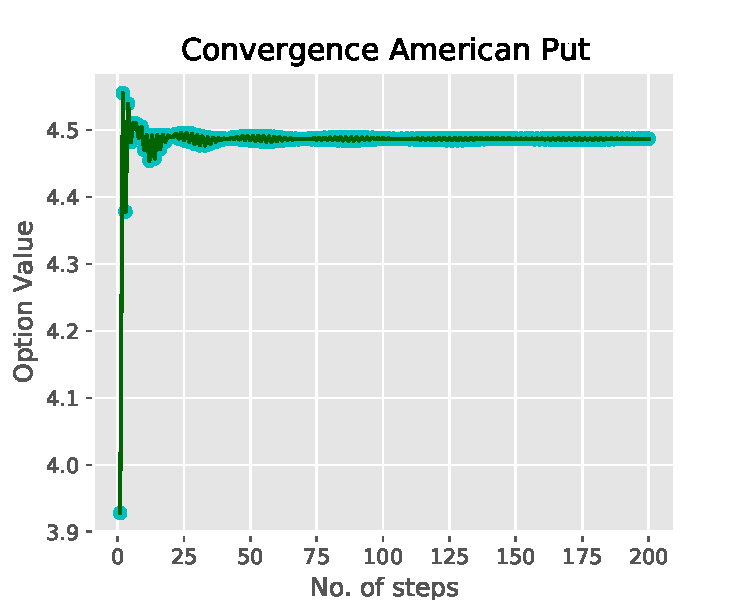
\includegraphics{Figures/binConv.pdf}
\decoRule
\caption[Convergence of Binomial Model]{Price for an American put option based on the binomial model, where the independent variable is the number of time-steps. Parameters are $T=1$, $K=40$, $S(0)$=40, $\sigma$=0.2, and $r=0.06$.}
\label{fig:binConv}
\end{figure}

We have seen the central concepts arbitrage and completeness from continuous time in action for the discrete time setup. The paper \parencite{CRR} which introduced the binomial model to option pricing came after the Black-Scholes model described in section \ref{Chapter2} \parencite{B-S-Paper}. The main reason for developing a binomial model is that the discrete time model gives a simplified model in terms of the mathematics and highlights the essential concepts in arbitrage theory. You can argue that the simpler mathematics in this model makes the binomial pricing method more instructive and clear. Besides being easier to understand for non-mathematicians, it works nicely with other options than the European options like American options. \\

Even though we assume the stock price moves at discrete jumps instead of lognormal returns in the continuous time model, it can actually be shown that the CRR binomial model will converge to the Black-Scholes model. Hence the binomial pricing model will be equivalent with the continuous time analytical pricing model derived by Fischer Black and Myron Scholes in the limit for European options. \\

The path-independence payoff for the American put makes the tree recombining, so there is only N+1 terminal nodes at maturity. If the derivative was path-dependent e.g. an Asian option, then we have a non-recombining tree and $2^{N}$ terminal nodes are needed. This is computationally inefficient, which explains that the binomial model should not be used for path-dependent derivatives. We will show below, that the intuitive CRR model can be extended to higher dimensions, but the model suffers from the curse of dimensionality.

\newpage
%----------------------------------------------------------------------------------------
%	SECTION 2
%----------------------------------------------------------------------------------------
\section{Binomial Lattice Model for Multivariate Contingent Claims}
We follow the approach in \parencite{BEG}, henceforth called the BEG method. The BEG method is a natural extension of the Cox Ross Rubinstein model (section \ref{CRR}) for multivariate contingent claims. The idea, as in the one dimensionel case, is to approximate the system of underlying processes\footnote{In Black-Scholes theory the stochastic process evolution for the stock is described by the GBM} with a discrete multivariate binomial lattice. The advantage is that for exotic options like the basket options the valuation of European put options is readily extended to American put options. \\

The BEG method has its limitation in terms of the number of underlying assets and for path dependent options (see section \ref{CRR}), but it is very intuitive. The problem with increasing the number of underlying assets is that the number of one-step transitions at each node is $2^d$ and the total number of terminal nodes after N steps is $(N+1)^d$ for path-independent derivatives. It means that the computational resources become an issue for high dimensional problems with the discrete time model approach. This makes the BEG method undesirable for options with many underlying assets. Another problem with three or more underlying assets is that some one-step transition probabilities can turn out negative with the BEG method, which makes the model nonsensical in those cases. For those reasons we choose to focus on the bivariate contingent claim i.e. $d=2$. \\

The model we want to approximate is the bivariate lognormal distribution, because we want to approximate the Black-Scholes model describing the evolution of the two risky assets (section \ref{MultiDimModel}). Under the risk neutral measure the SDE for the risky assets are:
$$dS_i(t)=S_i(t)r(t)dt+S_i(t)\sigma_i(t)dW^Q(t) \quad for \ i=1,2$$
We divide the time from inception to maturity into N equidistant intervals with length $\Delta t$. We want the jump distribution to approximate the continuous time bivariate lognormal distribution. Each time interval has a jump size defined in terms of the volatility and the length of the interval:
$$u_i=\exp(\sigma_i \sqrt{\Delta t}) \quad and \quad u_i \cdot d_i = 1 \quad for \ i=1,2$$
The $u_i$ and $d_i$ are the multiplication factors for the i'th stock, where the former is a jump up and the latter is a jump down factor for the stock. What is the probability that the stock jumps up or down? The probabilities are chosen such that the characteristic functions are equal for small time steps $\Delta t$ (p. 245-246 in \parencite{BEG} for details). The probabilities for the model with two underlying risky assets are:
\begin{equation}
\begin{split}
q_1=q_{uu}=\dfrac{1}{4}\bigg( 1+\rho + \sqrt{\Delta t}(\dfrac{\mu_1}{\sigma_1} + \dfrac{\mu_2}{\sigma_2}) \bigg)\\
q_2=q_{ud}=\dfrac{1}{4}\bigg( 1-\rho + \sqrt{\Delta t}(\dfrac{\mu_1}{\sigma_1} - \dfrac{\mu_2}{\sigma_2}) \bigg)\\
q_3=q_{du}=\dfrac{1}{4}\bigg( 1-\rho + \sqrt{\Delta t}(-\dfrac{\mu_1}{\sigma_1} + \dfrac{\mu_2}{\sigma_2}) \bigg)\\
q_4=q_{dd}=\dfrac{1}{4}\bigg( 1+\rho + \sqrt{\Delta t}(-\dfrac{\mu_1}{\sigma_1} - \dfrac{\mu_2}{\sigma_2}) \bigg)
\end{split}
\end{equation} 
The correlation $\rho$ between the two assets are assumed to be constant and $\mu_i=r-\frac{1}{2}\sigma_i^2$. We have illustrated below the evolution of binomial lattice model with two underlying risky assets, where we see that the number of nodes at maturity is $(1+N)^d$. 

\begin{figure}[th]
\centering
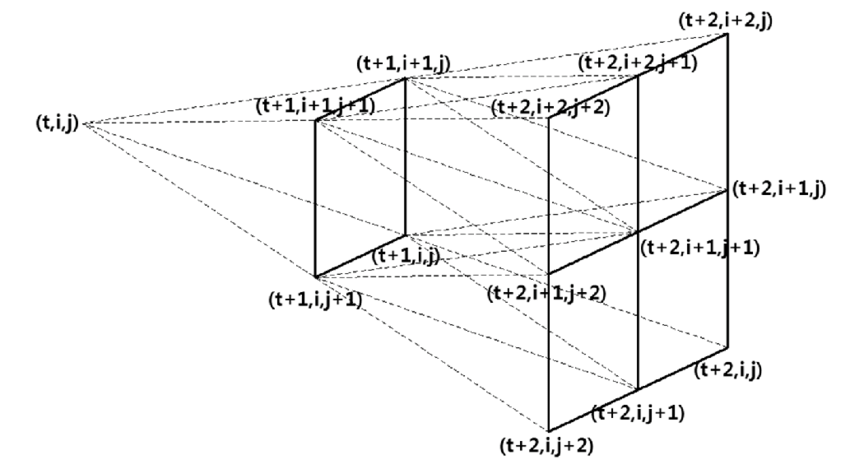
\includegraphics[width=\textwidth]{Figures/Three-dimensional-binomial-lattice.png}
\decoRule
\caption[Three-dimensional Binomial Lattice]{Evolution of binomial lattice model with two underlying risky assets, where t is time, i is number of up movements for $S_1$, and j is number of up movements for $S_2$. Figure is from the paper \parencite{KIM}}
\label{fig:threeDimLattice}
\end{figure}

After the construction of the evolution of the underlying assets, we can, like in the one-dimensional CRR model, recursively work backwards in the multidimensional binomial lattice. For the European option with $d$ underlying risky assets the recursive formula is:
$$J_{i_1,\ldots, i_d}(t_n)=\exp(-r\Delta t) \bigg(q_1 J_{i_1+1,\ldots, i_d +1}(t_{n+1}) + \cdots + q_{2^d} J_{i_1,\ldots, i_d}(t_{n+1}) \bigg)$$
Where $J$ is the value of the option to time $t_n$ and i is the number of times the underlying spot price at inception has been multiplied by u. For the American option the recursive formula is:
$$J_{i_1,\ldots, i_d}(t_n)=\max\{\Phi(t_n,\bm{S}(t_n)), \exp(-r\Delta t) \bigg(q_1 J_{i_1+1,\ldots, i_d +1}(t_{n+1}) + \cdots + q_{2^d} J_{i_1,\ldots, i_d}(t_{n+1}) \bigg)\}$$
With the recursive formulas we can valuate multivariate contingent claims for a variety of exotic options including the American put minimum of two stocks option. \\

The amount of computational required increases with the number of underlying assets for the binomial lattice methods. For the BEG method we have $2^d$ number of one-step transition probabilities. To reduce the number of transition probabilities, it has been tried in \parencite{NEK}, to set all the probabilities equal to 0.5 and then calculate the jump sizes. This is the reversed process compared to the BEG method, where the jump sizes are set first and then one-step probabilities are calculated. Choosing one-step probabilities and then the jump sizes has overcome the issue with negative probabilities for higher dimensions and in \parencite{NEK} the algorithm also seems to have faster convergence. The reserved approach of BEG is called the NEK approach.\\

The NEK and BEG approaches are both good in terms of both accuracy and computational speed for low dimensional option problems, but both still suffer from the curse of dimensionality. The simulations methods on the other hand, have somewhat of an advantage for higher dimensions. We choose to present the BEG approach, because it is a natural extension of the already presented CRR model, which we already built intuition upon. The key for the BEG approach is that we approximate a multivariate lognormal distribution with a discrete jump distribution. 

\newpage

\section{Least Squares Monte Carlo Method}\label{LSM}
We have seen that the binomial model is not suitable for path-dependent contingent claims like an Asian option and high dimensional multivariate contingent claims. Simulation methods overcome somewhat this issue. One of the first Monte Carlo methods for option pricing were to use pure simulation techniques. These methods overcame the issue of path-dependent option, but they still suffered the curse of dimensionality. To solve the dimensionality problem the LSM was born, where the idea is to combine simulation with regression. \\

A pure simulation technique has three ingredients: 
\begin{enumerate}
\item[•] A simulation based on the assumption of the underlying asset(s) distribution to price potential future prices
\item[•] From the simulation of the underlying asset(s) use the contract function to calculate the cash flow
\item[•] Discount back the cash flow to present value and average over the simulated paths
\end{enumerate}
The approach is suitable for the Asian option, because by simulation you have the whole path and averaging is straightforward. The pure simulation method would not be ideal for American options, because at each decision point for the American option, the pure simulation would need to simulate a new set of paths to estimate the expected continuation value. For reference of the pure simulation method see chapter 10 in \parencite{OVERHAUSMARCUS2007EHD}.\\ 

Remember, we approximate the American put option with a Bermudan put option for the simulation method. The simulation methods use the setup in section \ref{DiscreteValueFramework}. Again, we use dynamic programming to calculate the price of the American put option. The LSM algorithm overcomes the exponentially growing computational burden in pure Monte Carlo simulation by using regression to calculate the expected continuation value.

\subsection{The Algorithm}
To solve the optimal stopping problem numerically, we set up the mathematical framework for solving the problem inspired by \parencite{analysisLSM}. Remember the optimal stopping time problem in discrete time is:
\begin{equation}\label{Bermudanstop}
\sup_{\tau \in \mathcal{T}(0,\ldots,T)} E^Q[G(S(\tau))]
\end{equation}
where $\mathcal{T}(0,\ldots,T)$ is a class of all $(0,\ldots,T)$-valued stopping times and $\bigg(S(0),S(t_1), \ldots, S(t_N)=S(T)\bigg)$ is the underlying stochastic Markovian process describing e.g. stock price, volatility, average stock price, etc. The Markov chain $(S_{t_n})_{n=0,\ldots,N}$ has state space $(E, \mathcal{E})$. The Snell envelope is given by:
$$U(t_n)=\esssup_{\tau \in \mathcal{T}(t_n,\ldots,t_N)} E^Q[G(S(\tau))|\mathcal{F}_n]$$
The Markov property implies that:
$$E^Q[G(S(\tau_{t_{n+1}}))|\mathcal{F}_{t_n}]=E^Q[G(S(\tau_{t_{n+1}}))|S(t_n)]=f(S(t_n))$$ 
and we assume the initial state to be $S(0)=s$ and deterministic. We solve equation \eqref{Bermudanstop} by the theory presented in section \ref{DiscreteValueFramework}. Hence, the dynamic programming principle on the optimal policy is:
\begin{equation}\label{LSMDynamic}
\begin{split}
\begin{cases}
          \tau_{t_N} = t_N\\
          \tau_{t_n} = t_n \cdot 1_{\{G(S(t_n)) \geq E^Q[G(S(\tau_{t_{n+1}}))|S(t_n)])\}} + \tau_{t_{n+1}} \cdot 1_{\{G(S(t_n)) < E^Q[G(S(\tau_{t_{n+1}}))|S(t_n)])\}} \quad for \ n={0,\ldots,N-1} \\ 
\end{cases}
\end{split}
\end{equation}
Equation \eqref{LSMDynamic} involves many conditional expectations. Hence, we need an effective algorithm for evaluating them. The pure simulation methods were expensive, because the paths required for evaluating the series of conditional expectations increases exponentially with the number of exercise dates (chapter 10 \parencite{OVERHAUSMARCUS2007EHD}). The solution suggested e.g. in \parencite{LSM,Tsitsiklis} is to use the cross-sectional information in the simulated paths. The information is used for least squares regression. \\

The LSM algorithm approximates the expected continuation value with respect to $S(t_{n})$ by orthogonal projection on the state-space generated by finite number of basis functions of $S(t_{n})$. Define the sequence $(e_{j}(s))_{j\geq 1}$ of real measurable functions defined on the state space $(E,\mathcal{E})$. Assume:
\begin{enumerate}\label{AssumptionBasisFck}
\item[•] The sequence $(e_{j}(S(t_n)))_{j\geq 1}$ is total in $L^2(\sigma(S(t_n)))$ for $n=1,\ldots,N-1$.
\item[•] if $\sum_{j=1}^{m} \lambda_j e_{j}(S(t_n))=0 \ a.s.$ then $\lambda_j=0$ for $n=1,\ldots,N-1$, $m\geq 1$ and $j=1,\ldots,m$\\
\null \hfill (p. 3 \parencite{analysisLSM})
\end{enumerate}
By defining the vector space generated by $(e_{j}(s))_{j=1, \ldots, m}$ we denote the orthogonal projection from $L^2(\Omega)$ onto the vector space by $P^m_{t_n}$.
We approximate the expected continuation value by the projection:
\begin{equation*}\label{LSMDynamic2}
\begin{split}
\begin{cases}
          \tau_{t_N}^{[m]} = t_N\\
          \tau_{t_n}^{[m]} = t_n \cdot 1_{\{G(S(t_n)) \geq P^m_{t_n}(G(S(\tau^{[m]}_{t_{n+1}})))\}} + \tau^{[m]}_{t_{n+1}} \cdot 1_{\{G(S(t_n)) < P^m_{t_n}(G(S(\tau^{[m]}_{t_{n+1}}))) \}} \quad for \ n={0,\ldots,N-1} 
\end{cases}
\end{split}
\end{equation*}
Where:
$$P^m_{t_n}(G(S(\tau^{[m]}_{t_{n+1}})))=\alpha^{m}(t_{n}) \cdot e^m(S(t_{n})) \quad for \ n=1,\ldots,N-1$$
and the $\cdot$ on the right hand side is the inner product in $\mathbb{R}^m$ and $e^m=(e_1,\ldots, e_m)$.
By solving the above dynamic programming equation the time 0 approximate price of the Bermudan option is:
$$U^m(0)=\max \{ G(S(0)), E^Q[G(S(\tau^{[m]}_{t_1}))]\}$$
Where $G(S(0))$ is deterministic by assumption, but $E^Q[G(S(\tau^{[m]}_{t_1}))]$ needs to be evaluated numerically. In the LSM algorithm the methods for evaluating the projection is Monte Carlo simulation.\\

From the assumption about the distribution of the underlying state space we simulate K independent paths $S^{(1)}(t_n), S^{(2)}(t_n), \ldots, S^{(k)}(t_n), \ldots, S^{(K)}(t_n)$ of the Markov chain $S(t_n)$ with gain process $G(S^{(k)}(t_n))$ for $k=1, \ldots, K$ and $n=0,\ldots,N$. The least squares estimator $\alpha^{(m,K)}(t_n)\in \mathbb{R}^m$ for the simulated paths is:
\begin{equation}\label{LSMestimator}
\alpha^{(m,K)}(t_n)= \argmin_{a\in \mathbb{R}^m} \sum_{k=1}^{K} \bigg(G(S^{(k)}(\tau^{k,m,K}_{t_{n+1}}))  -a \cdot e^m(S^{(k)}(t_{n})) \bigg)^2 \quad for \ n=1, \ldots, N-1
\end{equation}
Where the recursively estimated stopping time is defined by:
\begin{equation*}\label{LSMDynamic3}
\begin{split}
\begin{cases}
          \hat{\tau}_{t_N}^{k,m,K} = t_N\\
          \hat{\tau}_{t_n}^{k,m,K} = t_n \cdot 1_{\{G(S^{(k)}(t_n)) \geq \alpha^{m,K}(t_{n}) \cdot e^m(S^{(k)}(t_{n})) \}} + \hat{\tau}_{t_{n+1}}^{k,m,K} \cdot 1_{\{G(S^{(k)}(t_n)) < \alpha^{m,K}(t_{n}) \cdot e^m(S^{(k)}(t_{n})) \}} \quad for \ n={0,\ldots,N-1} \\ 
\end{cases}
\end{split}
\end{equation*}
An example of polynomial regression on each exercise date is illustrated in figure \ref{fig:LSM1}, where the blue line is the estimated expected continuation value. From following the optimal stopping strategy by dynamic programming we derive the approximation for $U^{m}(0)$ from the simulated paths. The time 0 approximate price of the Bermudan option is:
\begin{equation*}
U^{m,K}(0) = \max \{ G(S(0)), \frac{1}{K} \sum_{k=1}^{K} G(S^{(k)}(\hat{\tau}^{k,m,K}_{t_1}))]\}
\end{equation*}

\begin{figure}[th]
\centering
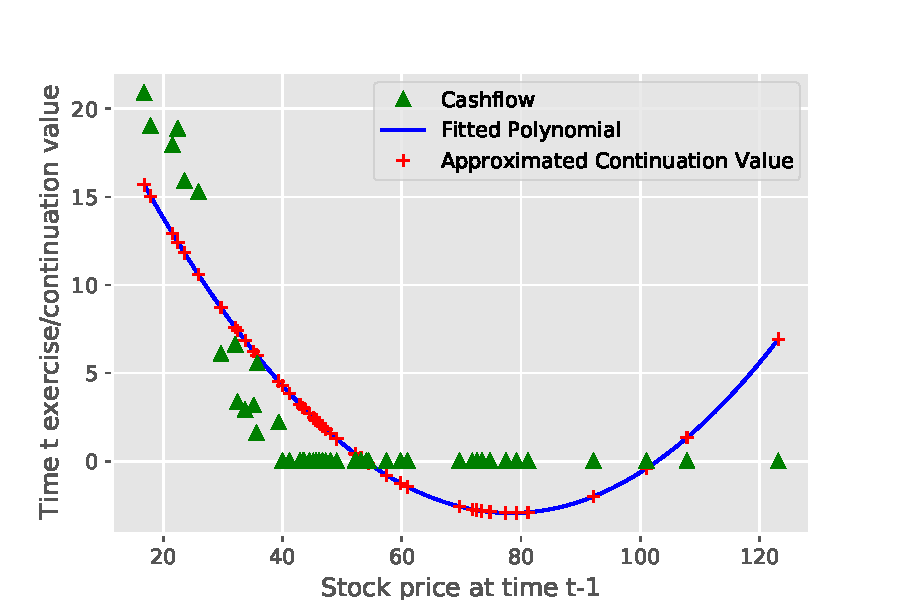
\includegraphics{Figures/LSMFit1.pdf}
\decoRule
\caption[Polynomial Regression of Continuation Value]{By zooming in on a specific point of time in the dynamic programming approach, we see how the algorithm regress the continuation value. In the illustration we used a quadratic polynomial regression model}
\label{fig:LSM1}
\end{figure}

\subsection{American Put}
The optimal stopping problem for an American put 
\begin{equation*}\label{optimalStopPut}
\begin{split}
P(0,s) = \sup_{\tau \in \mathcal{T}(0,\ldots,T)} E_{s}^Q[ \exp(-r \tau) \cdot \max\{K-S(\tau), 0 \}]
\end{split}
\end{equation*}
can be solved with the LSM algorithm. The stock values are modeled via Black-Scholes theory\footnote{Illustration of generated path for the GBM in figure \ref{fig:BM}}, hence, the simulated evolution for the stock under the risk neutral valuation is given by:
\begin{equation*}
\begin{split}
S(t)=S(0) \cdot \exp \bigg( (r -\frac{1}{2} \sigma^2) t + \sigma W(t) \bigg)
\end{split}
\end{equation*}
The stock paths are simulated from inception up to maturity with N+1 exercise dates. The focus in this section is on a univariate contingent claim and for convenience we assume the risk-free interest rate and the volatility are constants. As in the binomial model, we first construct the paths and then work backwards from maturity to inception at each exercise date to decide the optimal stopping time. \\

From previously, we know the dynamic programming principle on optimal policy gives the first optimal stopping time and at each decision point we regress the expected payoff by continuation of the contract and compare it to the intrinsic value. The dependent variable in the regression is the expected value of continuation and the independent variables are a set of orthogonal basis functions in $L^2(\sigma(S(t_n)))$ of the simulated paths. Typical choices for basis functions could be weighted Laguerre -, Hermit -, and Jacob polynomials. The weighted Laguerre polynomial is given by:
\begin{align*}
e_0(S) &= \exp(-S/2) \\
e_1(S) &= \exp(-S/2) (1-S) \\
e_2(S) &= \exp(-S/2) (1-2S+S^2/2) \\
\vdots \\
e_j(S) &= \exp(-S/2) \dfrac{\exp(S)}{j!} \frac{d^j}{dS^j}(S^j \exp(-S)) 
\end{align*} 
This kind of regression is a nonlinear expansion of the linear model\footnote{Prediction is a linear function of the coefficients}. We define regressed conditional expectation by:
$$\Psi(S(t_n); \alpha)= \sum_{j=0}^p \alpha_j \cdot e_j(S(t_n)) $$
where $\alpha$ is the coefficient for the regression, e is the basis function, where the argument is the underlying Markovian process $S$. By using this iterative method, we arrive at the pathwise optimal stopping policy, where in figure \ref{fig:LSM2} an example of pathwise optimal stopping times are shown. The figure illustrates that the option only can be exercised once, hence, the white lines after the triangles.\\

\begin{figure}[th]
\centering
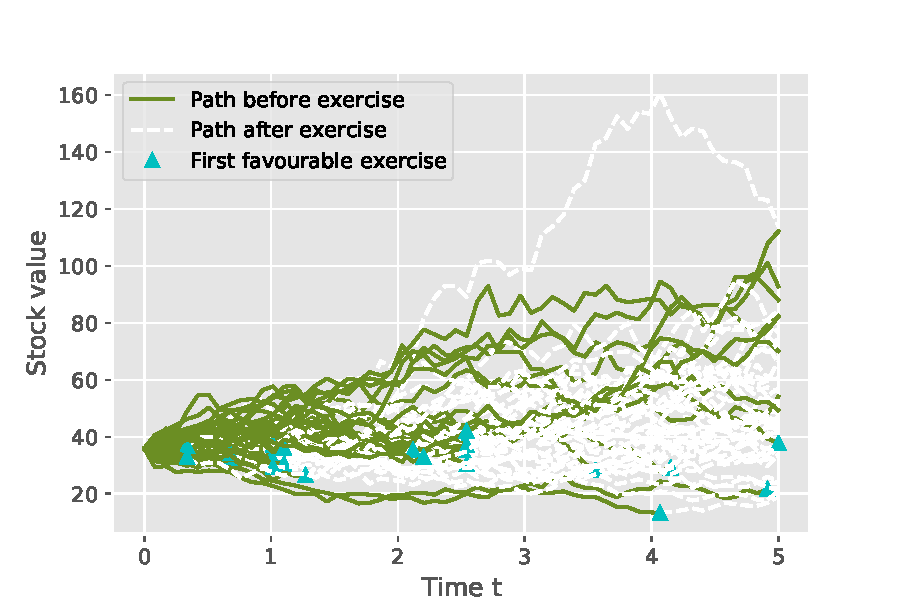
\includegraphics{Figures/LSMFit2.pdf}
\decoRule
\caption[Optimal Stopping Decision]{The optimal stopping decisions by the least squares Monte Carlo method}
\label{fig:LSM2}
\end{figure}

Note that for practical implementation the LSM is only considered in the money path. Hence, equation \eqref{LSMestimator} is changed to:
\begin{equation*}
\alpha^{(m,K)}(t_n)= \argmin_{a\in \mathbb{R}^m} \sum_{k=1}^{K} 1_{\{G(S^{(k)}(t_n))>0\}} \bigg(G(S^{(k)}(\tau^{k,m,K}_{t_{n+1}}))  -a \cdot e^m(S^{(k)}(t_{n})) \bigg)^2 \quad for \ n=1, \ldots, N-1
\end{equation*}
Therefore, only the in the money (ITM) paths are used for regression. Using only the ITM paths improves the algorithm, because the option value can never be less than zero, but including the other paths can yield negative results. The two articles \parencite{LSM, Tsitsiklis} have some differences in their approaches. The LSM considers only ITM and uses policy iteration instead of value iteration. Furthermore, in \parencite{Tsitsiklis} they set $U(t_n)= \Psi(S(t_n); \alpha)$ instead of $U(t_n)= U(t_{n+1})$ as in the LSM. These design choices make the LSM the most used method and it has the highest accuracy.\\

Note, for our computational implementation we use the same paths for decision making and valuation, this gives a biased high, but the difference in practice is not noticeable. In general the LSM is biased low, because of the sub-optimal exercise strategy\footnote{The LSM algorithm gives a lower bound see in appendix \ref{LSMLowerBound}}. Therefore, an upper bound can be computed for the option price, which is done in \parencite{AndersenLeif2004}. We wrap up the LSM section by looking at how the method can be used for basket options.

\subsection{Pricing Multivariate Contingent Claims with LSM}\label{LSMExtension}
For pricing of bivariate and multivariate contingent claims, we have to account for correlation between assets. The correlation matrix $\bm{\rho}$ is given by:
\begin{equation*}
\bm{\rho} = \begin{pmatrix}
\rho_{1,1} & \rho_{1,2} & \cdots & \rho_{1,d} \\
\rho_{2,1} & \rho_{2,2} & \cdots & \rho_{2,d} \\
\vdots & \vdots & \ddots & \vdots \\
\rho_{d,1} & \rho_{d,2} & \cdots & \rho_{d,d} \\
\end{pmatrix} = \begin{pmatrix}
1 & \rho_{1,2} & \cdots & \rho_{1,d} \\
\rho_{2,1} & 1 & \cdots & \rho_{2,d} \\
\vdots & \vdots & \ddots & \vdots \\
\rho_{d,1} & \rho_{d,2} & \cdots & 1 \\
\end{pmatrix}
\end{equation*}
The correlation between assets is given by $(\rho_{i,j})_{i\neq j}$ and each asset has correlation 1 with itself. We assume that $(\rho_{i,j})_{i \neq j} \in (-\frac{1}{d-1},1]$, because then the correlation matrix is a real, symmetric, and positive definite. Hence, Cholesky factorization can be utilized $\bm{\rho}=\matr{L}\matr{L}^T$ where $\matr{L}$ is a lower triangular matrix. From the decomposition it is easy to simulate correlated assets in d-dimensional Black-Scholes model:
\begin{equation*}
dS_{i}(t)=S_{i}(t) r dt + S_{i}(t) \sigma_i \matr{L}_{i,:} d\bm{W}(t) \quad i \in \{1,2,\ldots, d\}
\end{equation*}
Where $\bm{W}$ lies in $\mathbb{R}^d$ and $\bm{\sigma}=(\sigma_1, \sigma_2, \ldots, \sigma_d)$ is a vector of volatilities.\\

By simulating the paths according to the Black-Scholes dynamic, it is straightforward to apply the LSM for multivariate contingent claims, because it follows the same algorithm just with a different contract function.\\

Note in the next section, it will be more convenient to work with the covariance matrix $\Sigma$ and the covariance matrix is given by:
$$\Sigma=D(\bm{\sigma}) \bm{\rho} D(\bm{\sigma})$$
The Cholesky factorization is then:
$$\Sigma=\matr{A}\matr{A}^T$$

\newpage

%----------------------------------------------------------------------------------------
%	SECTION 4
%----------------------------------------------------------------------------------------

\section{Closed Form Solutions for European Exotic Options}\label{ExoticEuro}
Most exotic options require numerical methods, but in some special cases there exist a closed form solution. We will look at some of them in this section, where the purpose is to provide benchmarks for the numerical methods. Furthermore, we explore the boundaries of closed form solutions and show applications of martingale theory. Throughout the financial market and model assumptions given in section \ref{FinMarket} and \ref{MultiDimModel} will be assumed. We derive closed form solutions to European call and put options depending on several variables, for simplicity we will focus on pricing options with two or three underlying stocks. The section is inspired by the article \parencite{Ouwehand2006}. The exotic contingent claims we will consider are the geometric mean -, maximum - and minimum call option.

\subsection{Geometric Mean Basket Call Option}\label{GeoBasket}
For a geometric mean basket call option the contract function is given by:
\begin{align*}
\Phi(\bm{S}(T))=\max\{ (\prod_{i=1}^{d} S_i(T))^{\frac{1}{d}}-K,0 \}
\end{align*}
The key to  derive a closed form solution is the known result that the sum of normal random variables is multivariate normally distributed.
This implies that the product of lognormal random variables are multivariate lognormally distributed, since: 
\begin{equation*}
\begin{split}
\exp(x+y)&=\exp(x)\cdot \exp(y) \\
& \text{and}\\
 X \sim \mathcal{N}(\mu,\sigma^2) & \Rightarrow Y = \exp(X)\sim LN(\mu, \sigma^2)
\end{split}
\end{equation*}

Remember the assumption in section \ref{MultiDimModel} that the stock price process follows a GBM, hence:
\begin{equation}\label{prodGBM}
\begin{split}
(\prod_{i=1}^{d} S_i(T))^{\frac{1}{d}} = (\prod_{i=1}^{d} S_i(0))^{\frac{1}{d}} \exp\bigg((r-\frac{1}{2d}\sum_{i=1}^{d}\sigma_i^2)T + \frac{1}{d} \sum_{i=1}^{d} \sigma_i W_i(T) \bigg)
\end{split}
\end{equation}
Define:
\begin{align*}
\tilde{\sigma} = \frac{1}{d} \sqrt{\sum_{i=1}^{d} \sigma_i^2 + 2 \sum_{i\neq j} \rho_{i,j} \sigma_i \sigma_j}\\
F=(\prod_{i=1}^{d} S_i(0))^{\frac{1}{d}} \exp\bigg((r-\frac{1}{2d}\sum_{i=1}^{d}\sigma_i^2)T + \frac{1}{2} \tilde{\sigma}^2 \cdot T \bigg)\\
\epsilon = \frac{\frac{1}{d} \sum_{i=1}^{d} \sigma_i W_i(T)}{\tilde{\sigma} \sqrt{T}} \sim \mathcal{N}(0,1)
\end{align*}
and rewrite equation \eqref{prodGBM} by above definitions:
$$(\prod_{i=1}^{d} S_i(T))^{\frac{1}{d}} = F \cdot \exp\bigg( -\frac{1}{2} \tilde{\sigma}^2 \cdot T + \tilde{\sigma} \sqrt{T} \epsilon \bigg)$$
This expression is one-dimensional and is the standard GBM solution with zero drift and spot F. This has a known solution with Black-Scholes theory (section \ref{classicBS}) and the geometric mean call option has price
\begin{equation*}
\Pi(t,\mathcal{X})=\exp(-r \cdot (T-t))\bigg(F N(d_1) - K N(d_2) \bigg)
\end{equation*}
where $d_1=\frac{\ln(\frac{F}{K}) + \frac{1}{2} \tilde{\sigma}^2 T}{\tilde{\sigma} \cdot \sqrt{T}}$ and $d_2=d_1-\tilde{\sigma} \sqrt{T}$\\

The fact that the sum of normal random variables is multivariate normally distributed makes the geometric mean option easy to price in the Black-Scholes model, because the high dimensional problem can be treated as a one-dimensional problem.

\subsection{Options on the Maximum or the Minimum of Several Assets}
Here we restrict ourselves to consider the case with three underlying stocks like in \parencite{Ouwehand2006}, but the formula can be generalized to higher dimensions. The contract functions we consider are:
\begin{enumerate}
\item[•] Best of assets: $\Phi(S(T))=\max\{S_1,S_2,\ldots,S_{d}\}$
\item[•] Best of assets or cash: $\Phi(S(T))=\max\{S_1,S_2,\ldots,S_{d-1},K\}$
\item[•] Call on maximum: $\Phi(S(T))=\max\{\max(S_1,S_2,\ldots,S_{d-1})-K,0\}$
\item[•] Call on mininum: $\Phi(S(T))=\max\{\min(S_1,S_2,\ldots,S_{d-1})-K,0\}$
\end{enumerate}
Assume WLOG $d$=4 to avoid cumbersome calculations and notation. The section will heavily use the martingale framework developed in section \ref{MultiDimModel} and stochastic calculus (Appendix \ref{AppendixA}) to value these exotic options. The key is to choose the numéraire to a risky asset instead of the bank account. By results from section \ref{MultiDimModel} the processes are still Q-martingales given the numéraire is strictly positive. Under the assumption of an arbitrage-free and complete market it follows from risk neutral valuation formula:
$$S_0(t)E^{Q_0}_t[\frac{X}{S_0(T)}]=S_1(t)E^{Q_1}_t[\frac{X}{S_1(T)}]$$
This shows that changing the numéraire does not change the price of the derivative.

\subsubsection{Best of Assets or Cash}
The best of assets option will provide the foundation for pricing best of assets or cash and call on maximum or minimum options. The best of assets derivative pay out the price of the most valuable asset. The idea is then to set up 4 derivatives, where each derivative only gives a payout if the underlying stock is the most valuable out of the four stocks. This can be written with an indicator, where the payoff for the $i$'th asset is:
\begin{equation}\label{ithPayoff}
S_i(T) \cdot 1_{\{S_i(T)>S_j(T): i\neq j\}} \quad i=\{1,2,3,4\}
\end{equation}

From equation \eqref{ithPayoff} we see that the i'th asset is only different from zero, when it is the most valuable asset. The fair price for best of assets option $\Pi_{max}(t,\mathcal{X})$ is then given as the sum of the 4 derivatives. Hence, the best of asset derivative can be found by applying RNVF (proposition \ref{RNVF}) for each of them.\\

Let us first consider i=1 and we set $S_1$ to be the numéraire asset with martingale measure $Q_1$. Then by RNVF:
\begin{equation}\label{ithDerivative}
\begin{split}
\Pi_1(t, \mathcal{X})&=S_1(t)E_t^{Q_1}[1_{\{S_1(T)>S_2(T), S_1(T)>S_3(T), S_1(T)>S_4(T)\}}]\\
&=S_1(t) Q_1[\ln(\frac{S_2(T)}{S_1(T)})<0, \ln(\frac{S_3(T)}{S_1(T)})<0, \ln(\frac{S_4(T)}{S_1(T)})<0]
\end{split}
\end{equation}
From the above discussion the derivative price can be found by cycling through the 4 derivatives. Equation \eqref{ithDerivative} can be evaluated, therefore we seek to evaluate the probability under the $Q$-martingale measure. By Ito's lemma (see \ref{Ito}) the discounted process with stock j is:
\begin{align*}
d(\dfrac{S_i(t)}{S_j(t)})=\frac{S_i(t)}{S_j(t)} \cdot (a_i-a_j)dW^{Q_j}(t) 
\end{align*}
where $dW^{Q_j}(t)$ is standard d-dimensional $Q_j$-Wiener process and $a_i$ is the i'th row of the matrix $\matr{A}$ given in section \ref{LSMExtension}. \\

From the known solution of the GBM we have the distribution.
\begin{align*}
\ln(\frac{S_i(T)}{S_j(T)})\sim \mathcal{N}\bigg(\ln(\frac{S_i(t)}{S_j(t)}) - \frac{1}{2}\sigma_{i/j}^2 \cdot (T-t), \sigma_{i/j}^2 (T-t)\bigg)
\end{align*}
where $\sigma_{i/j}=(a_i-a_j)$ and $\sigma_{i/j}^2=\sigma_i^2+\sigma_j^2-2\rho_{ij}\sigma_i \sigma_j$.\\

Besides using the definition for $d_1$ and $d_2$ in proposition \ref{BS-price-EuroCall} we define:
\begin{align*}
d^{i/j}_1 =\frac{1}{\sigma_{i/j}\cdot \sqrt{T-t}} \cdot \bigg( \ln(\frac{S_i(t)}{S_j(t)}) + \frac{1}{2} \sigma_{i/j}^2 \cdot (T-t) \bigg)\\
d^{i/j}_2=d^{i/j}_1-\sigma_{i/j} \sqrt{T-t}
\end{align*}
The correlation between $\frac{S_i(T)}{S_k(T)}$ and $\frac{S_j(T)}{S_k(T)}$ is:
\begin{align*}
\rho_{ij,k}&:= \dfrac{(a_i-a_k)\cdot(a_j-a_k)}{||a_i-a_k|| \cdot ||a_j-a_k||}\\
&=\frac{\rho_{ij}\sigma_i \sigma_j - \rho_{ik}\sigma_i \sigma_k - \rho_{kj}\sigma_k \sigma_j + \sigma_k^2}{\sqrt{(\sigma_i^2 + \sigma_k^2 - 2\rho_{ik}\sigma_i \sigma_k)\cdot(\sigma_j^2 + \sigma_k^2 - 2\rho_{jk}\sigma_j \sigma_k)}}
\end{align*}
Hence:
$$Q_1[\ln(\frac{S_2(T)}{S_1(T)})<0, \ln(\frac{S_3(T)}{S_1(T)})<0, \ln(\frac{S_4(T)}{S_1(T)})<0]=N_3(-d_2^{2/1},-d_2^{3/1},-d_2^{4/1}, \rho_{23,1}, \rho_{24,1}, \rho_{34,1})$$
Cycling through each derivative, we get:
\begin{equation}\label{BestAsset}
\begin{split}
\Pi_{max}(t,\mathcal{X})&=S_1(t) N_3(-d_2^{2/1},-d_2^{3/1},-d_2^{4/1}, \rho_{23,1}, \rho_{24,1}, \rho_{34,1}) \\
&+S_2(t) N_3(-d_2^{1/2},-d_2^{3/2},-d_2^{4/2}, \rho_{13,2}, \rho_{14,2}, \rho_{34,2})\\
&+S_3(t) N_3(-d_2^{1/3},-d_2^{2/3},-d_2^{4/3}, \rho_{12,3}, \rho_{14,3}, \rho_{24,3}) \\
&+S_4(t) N_3(-d_2^{1/4},-d_2^{2/4},-d_2^{3/4}, \rho_{12,4}, \rho_{13,4}, \rho_{23,4})
\end{split}
\end{equation}
We can extend the above result to best of assets and cash by letting $S_4(t)=K\exp(-r(T-t))$, where K does not have any volatility and is also independent of the other assets, hence, equation \eqref{BestAsset} becomes:
\begin{equation*}\label{BestAssetOrCash}
\begin{split}
\Pi_{max}(t,\mathcal{X})&=S_1(t) N_3(-d_2^{2/1},-d_2^{3/1},d_1^{1}, \rho_{23,1}, \rho_{24,1}, \rho_{34,1}) \\
&+S_2(t) N_3(-d_2^{1/2},-d_2^{3/2},d_1^{2}, \rho_{13,2}, \rho_{14,2}, \rho_{34,2})\\
&+S_3(t) N_3(-d_2^{1/3},-d_2^{2/3},d_1^{3}, \rho_{12,3}, \rho_{14,3}, \rho_{24,3}) \\
&+K\cdot \exp(-r(T-t)) N_3(-d_2^1,-d_2^2,-d_2^3, \rho_{12}, \rho_{13}, \rho_{23})
\end{split}
\end{equation*}

\subsubsection{Call on Max and Call on Min}
From the price of the best of asset or cash option can the call max option price be derived. Note that:
$$\max\{\max\{ S_1,S_2,S_3 \} - K, 0\}=\max\{\max\{ S_1,S_2,S_3 \}, K\} - K = \max\{ S_1,S_2,S_3,K \} - K$$
The call on max option is then a best of asset or cash option subtracted the strike. Realizing that fact, it is easy to price the call on max:
\begin{equation*}\label{callMax}
\begin{split}
\Pi_{cmax}(t,\mathcal{X})&=S_1(t) N_3(-d_2^{2/1},-d_2^{3/1},d_1^{1}, \rho_{23,1}, \rho_{24,1}, \rho_{34,1}) \\
&+S_2(t) N_3(-d_2^{1/2},-d_2^{3/2},d_1^{2}, \rho_{13,2}, \rho_{14,2}, \rho_{34,2})\\
&+S_3(t) N_3(-d_2^{1/3},-d_2^{2/3},d_1^{3}, \rho_{12,3}, \rho_{14,3}, \rho_{24,3}) \\
&-K \exp(-r(T-t)) \cdot\bigg(1 - N_3(-d_2^1,-d_2^2,-d_2^3, \rho_{12}, \rho_{13}, \rho_{23})\bigg)
\end{split}
\end{equation*}

Similar ideas are needed to derive the call on min, which we will not provide\footnote{The interested reader can read more on p. 6 in \parencite{Ouwehand2006}}. The fair price for the call on min derivative is:
\begin{equation*}\label{callMin}
\begin{split}
\Pi_{cmin}(t,\mathcal{X})&=S_1(t) N_3(d_2^{2/1},d_2^{3/1},d_1^{1}, \rho_{23,1}, -\rho_{24,1}, -\rho_{34,1}) \\
&+S_2(t) N_3(d_2^{1/2},d_2^{3/2},d_1^{2}, \rho_{13,2}, -\rho_{14,2}, -\rho_{34,2})\\
&+S_3(t) N_3(d_2^{1/3},d_2^{2/3},d_1^{3}, \rho_{12,3}, -\rho_{14,3}, -\rho_{24,3}) \\
&-K \exp(-r(T-t)) \cdot N_3(d_2^1,d_2^2,d_2^3, \rho_{12}, \rho_{13}, \rho_{23})
\end{split}
\end{equation*}

To derive the put of the exotic European options we can utilize a put-call-parity (p. 6 \parencite{Ouwehand2006}), but it takes a different form than the one presented in chapter \ref{Chapter2} proposition \ref{put-call-parity}. The put-call-parity for the exotic European call options is:
\begin{equation*}\label{putMin}
V_c(K)+K\exp(-r\cdot (T-t)) = V_p(K)+V_c(0)
\end{equation*}
Where $V_c(K)$ is the value of the exotic European call option.\\

The exotic European options serve as an benchmark for the multivariate lattice approach, because if the lattice approach is close to the European benchmark then it is reasonable to expect a close estimate to the American option. The above section is also a presentation of the martingale theory's versatility. 



